% !TeX encoding = UTF-8
% !TeX program = pdflatex
% !BIB program = biber

\documentclass[english]{lni}

\usepackage[
    backend=biber,
    style=LNI,
]{biblatex}
\addbibresource{references.bib}

\usepackage{algorithmic}
\usepackage{graphicx}
\usepackage{textcomp}
\usepackage{listings}
\usepackage{xcolor}
\usepackage{float}

\definecolor{codegreen}{rgb}{0,0.6,0}
\definecolor{codegray}{rgb}{0.5,0.5,0.5}
\definecolor{codepurple}{rgb}{0.58,0,0.82}
\definecolor{backcolour}{rgb}{1,1,1}

\lstdefinestyle{mystyle}{
    backgroundcolor=\color{backcolour},
    commentstyle=\color{codegreen},
    keywordstyle=\color{magenta},
    numberstyle=\tiny\color{codegray},
    stringstyle=\color{codepurple},
    basicstyle=\ttfamily\footnotesize,
    breakatwhitespace=false,
    breaklines=true,
    captionpos=b,
    keepspaces=true,
    numbers=left,
    numbersep=5pt,
    showspaces=false,
    showstringspaces=false,
    showtabs=false,
    tabsize=2,
    frame=single,
    xleftmargin=2em,
    framexleftmargin=1.57em,
    framexrightmargin=-0.5em
}

\lstset{style=mystyle}

\begin{document}
\title{Finding Concurrency Bugs in Production}
\author[Marvin Strangfeld]
{Marvin Strangfeld\footnote{RWTH Aachen University, \email{marvin.strangfeld@rwth-aachen.de}}}
\editor{Gesellschaft für Informatik} % Names of Editors
\booktitle{SKILL 2022} % Name of book title
\yearofpublication{2022}
%%%\lnidoi{18.18420/provided-by-editor-02} % if known
\maketitle

\begin{abstract}
Bugs that are caused by the parallel execution of a program, so called
concurrency bugs are often hard to find and therefore hard to fix.
In this paper we evaluate different techniques and tools that are currently available to effectively find, fix and avoid concurrency bugs.
These tools are evaluated by their ease of use, their computational and storage overhead, their concurrency bug coverage and their potential amount of false-positive reports.
The goal is to find tools that are production-ready and applicable to real-world software projects.
\end{abstract}
\begin{keywords}
    Software testing and Debugging \and
    Concurrent programming languages
\end{keywords}
%%% Beginn des Artikeltexts
\section{Introduction}

\begin{quote}
``Everyone knows that debugging is twice as hard as writing a program in the first place. So if you're as clever as you can be when you write it, how will you ever debug it?'' --- Brian W. Kernighan\cite{kernighan1974elements}
\end{quote}

\subsection{Heisenbugs}

% Motivation
Today's computer architectures rely more and more on parallel computing.
Single-core processors were widely replaced by multi-core architectures optimized to run processes and threads concurrently.
To utilize the full performance of the given hardware, developers need to write their software with a high degree of parallelism.
In contrast to sequential programs which only follow one predictable path through the program code, concurrent programs can have multiple paths that are executed independently from each other.
Using threads that branch off from the main program path, it is possible to execute operations in parallel.
The order in which these threads are executed is determined by the operating system's scheduler.
The resulting order of thread executions is often referred to as \emph{thread interleavings}.
Because a developer, like the program itself, cannot predict what resources also need processing time on a machine, the concrete schedule has to be handled as non-predictable and therefore as non-deterministic.
This introduces the potential for bugs that would not occur in sequential programs due to non-determinism in the order of execution.
Such bugs can be very challenging to debug because they are not easily reproducible~\cite{tu2019go}.
Due to this complexity, it is no surprise that bugs that are related to concurrency and parallel program execution occur quite often~\cite{lu2008mistakes}.
But non-deterministic behavior also means that a bug that is only triggered when a certain pattern of thread interleavings appear cannot be reliably reproduced without knowing the schedule it appeared in.

In 1986 Jim Gray introduced the term ``Heisenbug'' for these kind of software failures.
He wrote:

\begin{quote}
``[...] Heisenbugs may elude a bugcatcher for years of execution. Indeed, the bugcatcher may perturb the situation just enough to make the Heisenbug disappear.''\cite{gray1986computers}
\end{quote}

Heisenbugs are bugs that only manifest within very specific thread interleavings that might not occur when a bugcatcher evaluates the program.
The complexity and uncertainty of concurrency bugs is also the reason for studies~\cite{tu2019go} that examine how these bugs occur and explore different ways on how to detect, fix and avoid them.
Thus, numerous tools and techniques have been developed that propose different solutions to solve the problem of concurrency bugs or accelerate the debugging process.

In this paper we evaluate some of these techniques and tools and how they can be used to ease the process of debugging concurrent bugs.
The main focus is to detect bugs efficiently in production, which means that developers should be able to fix bugs with a minimum amount of work and time.
Also, the manifestation of concurrency bugs should be reported immediately with minimal overhead of computational resources.
For all of this it is also desirable to have a maximum amount of coverage with only minimal false-positive reports.

\subsection{The Go Programming Language}
The increasing demand for parallel programs has also lead to the development of new programming languages which specialize in this task.
The goal of these languages is to ease the usage of parallel programming patterns, so developers can use them more often without writing extensively more code.
One example for such a language is Go which is a statically typed programming language developed by Google, that compiles down to native binaries~\cite{goDocs}.
Go recently gained a lot of popularity for the purpose of writing highly concurrent programs.
Popular open-source projects like \emph{Kubernetes}\footnote{\url{https://kubernetes.io/}}, \emph{Docker}\footnote{\url{https://www.docker.com/}} and \emph{Prometheus}\footnote{\url{https://prometheus.io/}} are all written in Go.
The official documentation of Go states: ``[... Go's] concurrency mechanisms make it easy to write programs that get the most out of multicore and networked machines [...]''~\cite{goDocs}.
Go abstracts the creation of threads by using lightweight \emph{goroutines}, which can be created by using the \lstinline{go} keyword followed by a named or anonymous function.
The Go runtime maps these goroutines to operating system threads during execution.
Go encourages programmers to use concurrency by \emph{message passing}, which is assumed to be safer and more convenient to use than \emph{shared memory}.
For this purpose Go is using a concept called \emph{channels} where typed messages can be passed through like a UNIX pipeline.
Beside the message passing however, it is also possible to make use of \emph{shared memory}, which gives the developer a lot of freedom to orchestrate the parallel execution of threads.
Even though Go is designed for programming concurrent programs, this does not mean that Go programs are free of concurrency bugs.
Projects written in Go also tend to have more concurrency than projects written in traditional programming languages such as C~\cite{tu2019go}.
So it is even more important for Go developers to catch concurrency bugs effectively and as early as possible.
Together with the increasing popularity of the language, the demand for production-ready tools to catch concurrency bugs is very high, which is why this paper evaluates existing techniques in the context of the Go programming language.

\subsection{Structure}

The further structure of this paper continues as follows:
\Cref{sct:taxonomy} gives a brief introduction on the different types of concurrency bugs and their main causes.
\Cref{sct:dynamic} covers some techniques to dynamically detect concurrency bugs and reliably reproduce them.
\Cref{sct:testing} shows different methods of concurrency-aware testing to detect concurrency bugs automatically in a testing environment, where in contrast to a production environment concurrency bugs are explicitly provoked.
Finally, \Cref{sct:static} covers how to detect concurrency bugs with static code analysis.


% ------------------------------------ %
% --- TAXONOMY OF CONCURRENCY BUGS --- %
% ------------------------------------ %
\section{Taxonomy of Concurrency Bugs}
\label{sct:taxonomy}

\begin{figure}
    \centering
    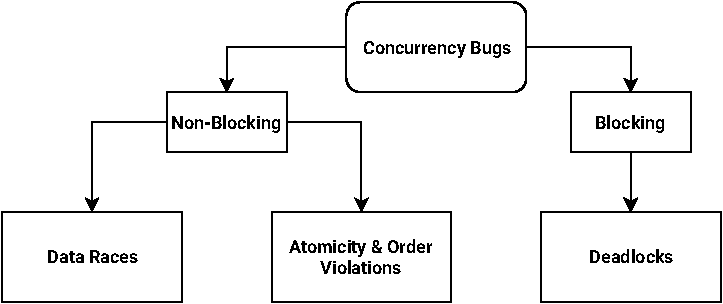
\includegraphics[width=0.7\linewidth]{figures/ConcurrencyBugClasses.pdf}
    \caption{A Taxonomy of Concurrency Bugs -- based on\cite{tchamgoue2012testing}}
    \label{fig:classes}
\end{figure}

\Cref{fig:classes} shows a taxonomy of concurrency bugs based on the work of Tchamgoue, Kim and Jun~\cite{tchamgoue2012testing}.
They distinguish between two main categories of concurrency bugs: \emph{Blocking} and \emph{non-blocking}.
Blocking bugs are bugs where the execution of a program is unintentionally blocked and the program cannot terminate.
The manifestation of these kind of bugs is very noticeable because the part of a program in which the deadlock appears in freezes and has to be restarted before the computation can continue.
Non-blocking bugs are often harder to find because they can occur even when the execution of a program does not block but the calculations are wrong.
This can also lead to a cascade of bugs where the root cause is a non-blocking concurrency bug which might not be obvious.

For example: A method concurrently creates a list of numbers that is expected to be ordered but due to a non-blocking concurrency bug the list suddenly contains unordered elements.
This failure might only occur once in a thousand executions or even less, due to the exponentially growing number of possible thread interleavings.
But if other methods depend on the correct order of the elements in this list, the program might crash or generate wrong results and the reason can be very hard to find.

\subsection{Deadlocks}

The most common manifestation of blocking bugs are \emph{deadlocks}, where circular dependencies between resources block the flow of a program.

\begin{lstlisting}[float=h, language=Go, label=lst:deadlockCh, caption={Deadlock caused by misuse of an \emph{unbuffered Channel}}]
func main() {
    data := make(chan int)
    done := make(chan bool)
    ch <- 1 // Program already blocks here
    go func() {
        process(<-data)
        done <- true
    }()
    <-done
}
\end{lstlisting}

An example of a deadlock in a Go program that might not be obvious is shown in \cref{lst:deadlockCh}, where unbuffered channels are used to transfer information between threads.
Go channels can either be buffered or unbuffered.
With unbuffered channels the sender thread has to wait until a second thread is ready to receive the message.
With buffered channels the message gets buffered and the sender thread can continue it's execution immediately as long as the buffer is not full.
In the first two lines of the main method of \cref{lst:deadlockCh}, the two unbuffered channels \lstinline{data} and \lstinline{done} are created to send data to the thread and to receive information when the execution of the thread is done.
Using the arrow notation, data can either be sent into a channel (line 4) or data can be received from a channel (line 6).
The bug in this case is that without an active listener on an unbuffered channel, any send action will be blocked.
To fix this, one could replace the unbuffered channel with a buffered one, so that the execution flow of the program can continue without blocking.
This shows how important it is to know the concrete implementation of a concurrency abstraction.
Even though intended to ease the synchronization between threads and make inter-thread communication safer, by not knowing the implementation of an abstraction the developer can unknowingly create hard to find concurrency bugs.

Another common problem in event-driven concurrent programs are \emph{blocking operations} like filesystem operations that are executed inside an event-handler.
Because event-handlers have a higher priority than non-event code, these operations can penalize and even paralyze the entire program execution~\cite{tchamgoue2012testing}.

\subsection{Data Races}

Data races are part of the non-blocking concurrency bugs.
They occur when multiple threads simultaneously try to access a shared variable where at least one access is a write operation~\cite{serebry2009threadsanitizer}.

\begin{lstlisting}[float=h, language=Go, label=lst:race, caption=Data race by concurrently accessing a map]
func main() {
	data := make(map[string]string)
	done := make(chan bool)
	go func() {
		data["1"] = "a" // First conflicting access.
		done <- true
	}()
	data["2"] = "b" // Second conflicting access.
	<-done
}
\end{lstlisting}

\Cref{lst:race} shows an example of a data race that is frequently found~\cite{serebry2009threadsanitizer}.
The data race happens when two threads access a non-thread-safe complex object (e.g. a map) without synchronization.
Even though the two threads in this example write to different keys of the map \lstinline{data}, this might cause a corruption of data or even crash the program because the default Go map implementation is not concurrency-aware.
To fix this, the access to the map needs to be synchronized, e.g. by a lock.

% TODO: Is it a data race or an atomicity violation?
A special case of data races are multi-variable data races.
In this case multiple variables that are semantically correlated are accessed by multiple threads and could therefore loose their semantic correctness when not handled correctly.
A common example for this are structs that have a data and a length field.
Whenever the data field gets updated, so does the length field which is semantically correlated with the data.
When multiple threads update these variables they need to synchronize not only on each of the variables separately but on all semantically correlated variables at the same time~\cite{lu2007muvi}.

\subsection{Atomicity and Order Violations}

Atomicity and order violations are concurrency bugs where the interleaving of threads violates the programmer's intention of atomicity and order.
\Cref{lst:order} shows a common order violation bug pattern called ``Test-and-Use''~\cite{farchi2003patterns}.
The programmer's intention is to check if a variable is not \lstinline{nil} and then use this variable.
However, due to the thread that was launched before, it could happen that after the \lstinline{if} check in line 7, the thread of the goroutine gets scheduled and the data variable is set to \lstinline{nil}.
To fix this bug, the check and the usage of the variable need to become an atomic operation to enforce the order of execution.

\begin{lstlisting}[float=h, language=Go, label=lst:order, caption=Test-and-Use bug pattern -- Order violation]
func main() {
    data := getData()
    go func() {
        process(data)
        data = nil
    }()
    if (data != nil) {
        process(data) // Might already be nil
    }
}
\end{lstlisting}

\begin{lstlisting}[float=h, language=Go, label=lst:atomicity, caption=Load-Store bug pattern -- Atomicity violation]
func main() {
    var group sync.WaitGroup
    group.Add(10)
    sum := 0
    for i = 0; i < 10; i++ {
        go func() {
            sum++ // Not atomic
            group.Done()
        }()
    }
    group.Wait()
}
\end{lstlisting}

\Cref{lst:atomicity} shows one example of the infamous ``Load-Store'' bug pattern~\cite{farchi2003patterns}.
The programmer might have assumed that \lstinline{++} is an atomic operation because it is one literal in Go.
However, after compilation, this is expanded to 3 instructions: LOAD, INCREMENT and finally STORE.
The thread scheduler could switch the context after any of these instructions.
This leads to unpredictable and non-deterministic behavior, when multiple threads try to increment the same variable.
To fix this bug pattern, the \lstinline{++} operation also needs to be replaced by an atomic operation that does not allow other threads to access the \lstinline{sum} variable while incrementing.


% ------------------------------------ %
% ------ DYNAMIC CODE ANALYSIS ------- %
% ------------------------------------ %
\section{Dynamic Code Analysis}
\label{sct:dynamic}

Assuming that a concurrency bug that rarely manifests, gets deployed into production.
How can it be found quickly?
And once reported, how can it be reproduced easily for debugging purpose?
One of the main techniques for finding concurrency bugs is dynamic code analysis.
In dynamic code analysis the runtime behavior of a program is observed to detect problematic patterns like un-synchronized variable accesses or deadlocks.
Assuming that a bug is reported that does not manifest regularly, this technique can help to find the manifestation of the bug more easily during the debugging process.
Additionally it could be used to observe deployments in production, so concurrency bugs get reported immediately as they occur.

\subsection{Record and Replay}
One popular dynamic code analysis technique is called ``Record and Replay'' where the path of execution of an application is recorded and can later be deterministically replayed.
To create a recording that contains all information to replay a program exactly the same way it was executed, the recorder needs to keep track of the schedule of the program as well as all variables that might not be deterministically reproducible.
Furthermore, any source of non-determinism such as the interaction with the network or graphics card or any call to external libraries needs to be recorded~\cite{lidbury2019sparse}.
This creates a lot of computational overhead in CPU time as well as storage.
This approach also forms the foundation for many other techniques and has many different variants and implementations~\cite{acm2002}~\cite{lidbury2019sparse}.

To track the schedule of a native binary application such as Go programs, the record tool has to sit between the host operating system and the application.
One requirement to use such a tool in production is the ease of deployability which means that the operational overhead should be very small.
There have been approaches with custom hardware or patched operating system kernels to hijack the scheduler, but these setups are quite complex and not easy to deploy~\cite{o2017engineering}.
One example for a tool that provides record and replay for native binary is \emph{rr}~\cite{mozillarr} developed by \emph{Mozilla}.
It does not need custom hardware and can run on an unmodified Linux operating system, which makes it easy to use and easy to deploy.
Their approach is to run the program to observe on a fixed CPU core and track the system calls by using \emph{ptrace}, which is a system call provided by the Linux kernel to inspect and observe processes.
This way they can record programs on an unmodified Linux system, which increases the deployability of such a setup.
With this approach they also do not need to modify the program itself with code instrumentation, where code is added to the program at compile time to observe it's runtime and which might affect the concurrency behavior.
The main performance bottleneck beside the execution on only one CPU core, are the context switches induced by ptrace~\cite{o2017engineering}.

Lidbury and Donaldson~\cite{lidbury2019sparse} examined further ways to reduce the computational overhead by a sparse recording approach.
By selectively ignoring ``unimportant'' sources of non-determinism, like the exact layout of memory, they were able to record input- and output-heavy applications like video games with a decreased overhead whereas \emph{rr} was not able to record at all due to the massive overhead of recording every source of non-determinism.
During replay they execute the thread schedule as recorded and mock every source of recorded non-determinism but let the ignored regions of the program execute non-deterministically.
Ignoring sources of non-determinism does decrease the accuracy in which concurrency bugs can be replayed.
But for real-world application one has to distinguish between the coverage of realistic bug occurrences and checking the overall correctness of a program.
In many cases it is more desirable to observe only one critical region of the code where concurrency bugs are either expected or could lead to serious issues than observing the entire program at once.
The right balance between coverage and overhead has to be individually evaluated by the safety and speed requirements of a program.
E.g. for a program that is used in a critical system like a banking environment, the developers should aim for a much higher coverage than for a regular web server, where speed is often more important than the overall correctness.

Sparse record and replay provides the ability to make these decisions and therefore adjust the needs to monitor applications in production.
Once a bug occurs and is either reported by a user or by the program itself, the developer could just replay the thread schedule to reproduce, find and therefore fix the bug quickly because, ``detecting concurrency bugs is difficult but once detected; correcting them is somehow an easy job''~\cite{tchamgoue2012testing}.
Additionally, this technique can help to reproduce all kinds of concurrency bugs, no matter if they are blocking or non-blocking.
For programs that do not heavily depend on parallelism this approach is also very feasible.
The tool \emph{rr} can record such programs with a performance overhead below the factor of two~\cite{o2017engineering}.
However, for programs that heavily rely on parallelism the overhead to record and store the thread schedule and all necessary parameters can decrease the performance by more than a factor of 30~\cite{o2017engineering}.
Especially for multi-threaded server applications that expect a high workload and where speed is crucial, this approach is not feasible in production.
And even if the workload is low but the application is time-sensitive for example because of protocol timeouts, it is not applicable without extending the acceptable timeouts.

\subsection{Data Race Detection}
Another set of tools for dynamic code analysis are dynamic data race detectors.
As the name implies, these tools detect data races but because atomicity and order violations are often correlated, these tools can detect a variety of non-blocking concurrency bugs.
There are multiple approaches for data race detection but in this case we refer to on-the-fly and post-mortem data race detection which are typically referred to as dynamic~\cite{serebry2009threadsanitizer}.
One data race detector that is mainly used for Go programs is the \emph{ThreadSanitizer} in version 2~\cite{threadSanitizer} developed by Google.
It is build into the Golang compiler tool-chain and can be toggled with a simple compiler flag which makes it very easy to use.
The tool performs compile-time instrumentation of the source program, in which all (atomic and non-atomic) accesses to potentially shared locations, as well as fence operations, are instrumented with calls into a linked run-time library~\cite{lidbury2019sparse}.
To distinguish between synchronized accesses and data races during runtime, the compiler also has to inject dynamic annotations into the program.
With these annotations the data race detector understands the synchronization primitives used by the programming language.
When the program along with the race detector gets executed, the data race detector observes the program execution as a sequence of events~\cite{serebry2009threadsanitizer}.
Each memory access is recorded and when receiving events for memory access it can report a potential race based on a state machine algorithm~\cite{serebry2011llvm}.

Performance-wise, race detection is unfortunately not better than the record and replay approach.
According to the official Go website: ``The cost of race detection varies by program, but for a typical program, memory usage may increase by 5-10x and execution time by 2-20x''~\cite{goRaceDetector}.
Which is in fact a massive improvement from \emph{ThreadSanitizer} version 1 with an overhead of 20x-50x, which was evaluated by Serebryany and Iskhodzhanov in 2009~\cite{serebry2009threadsanitizer}.
However, to improve this even further one possibility could be to ignore certain uncritical regions and just observe hotspots where data races are suspected, like in the sparse record and replay approach.
The overall coverage of data races would decrease but the developers could have the choice of balancing speed and correctness according to the requirements.

The main advantage of the dynamic approach is that it theoretically could be deployed to a real production environment.
For programs that are mainly event-driven this would give the ability to observe the real-world behavior in a reproducible way.
However, one of the main disadvantages of dynamic analysis tools is their bug coverage, that is typically small since only a few executions are explored~\cite{qadeer2004kiss}.
These tools just observe and do not actively try to enforce a manifestation of bugs, so not every thread interleaving might be explored.
Additionally, they depend on the the recognition of these bugs to report them correctly.
Programs that heavily rely on multi-threaded execution like web-servers can also become very inefficient or could even fail due to timeout limitations.
To avoid the overhead in the production environment and to find concurrency bugs in programs that could not be observed easily, it is desirable to find concurrency bugs before they can even get into production.


% ------------------------------------ %
% ---- CONCURRENCY-AWARE TESTING ----- %
% ------------------------------------ %
\section{Concurrency-aware Testing}
\label{sct:testing}

\begin{figure}
    \centering
    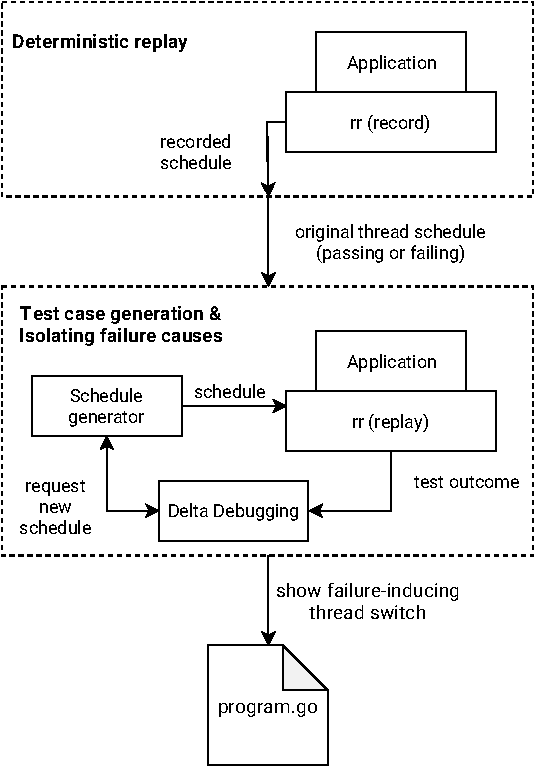
\includegraphics[height=0.4\textheight]{figures/Concurrency-Testing.pdf}
    \caption{Automatic concurrency-aware testing for Go programs -- based on\cite{acm2002}}
    \label{fig:testing}
\end{figure}

To prevent concurrency bugs to get into production and eventually causing damage, the software should be tested for those bugs before.
Extensive testing has proven to minimize the bugs of software in production~\cite{makinen2014testing}.
However, traditional testing mostly covers errors in sequential programs and cannot detect concurrency bugs effectively~\cite{lu2008mistakes}.
This lies in the nature of these bugs themselves.
When only certain thread interleavings trigger the bug, the tests could complete successfully almost every time without ever finding a manifestation.
For lack of established terms we will use the term \emph{concurrency-aware testing} to describe the process of automatically finding concurrency bugs in a testing environment by intentionally manipulating the path of execution.

One early attempt to test programs for concurrency bugs was to inject delays at random points in the program code~\cite{bron2005coverage}, but it is yet unclear if this heuristic really gives an acceptable bug coverage~\cite{lu2008mistakes}.
Furthermore, the tests should try to reduce the perturbation on the execution, so the software can be evaluated the same way as it would run in a regular deployment in production.

Another method of concurrency-aware testing has been proposed by Choi and Zeller~\cite{acm2002}.
They implemented a tool called ``DEJAVU''~\cite{acm2002} for the \emph{Jalapeño} Java Virtual Machine but the concept is also applicable to tools that work with Go or any other programming language.
They make use of a technique called \emph{Delta debugging}, which describes the process of narrowing down the spot where a failure is introduced by going back and forth between working and non-working conditions, in this case working and non-working thread schedules~\cite{zeller2002delta}.
By identifying the error-introducing thread switch, the corresponding unsafe operation of the program can be found.
\Cref{fig:testing} shows a modified model of the \emph{DEJAVU} approach, suited for Go programs by using rr instead of of \emph{DEJAVU} for the recording and replay of the thread schedule.
As a prerequisite, test cases need to be created that define the expected behavior of the application.
These can either succeed or fail which can be shown by the exit code for example.
In the first step, the Go application with these test cases gets executed and the thread schedule gets recorded by \emph{rr}.
The either failing or succeeding recorded thread schedule is then passed to the next instance where the delta debugging unit requests new executions of the application with an alternated thread schedule until it can pinpoint the failure-inducing thread switch.
The thread schedule is generated by the \emph{Schedule generator} and is replayed by the replay module in \emph{rr}.
The schedule as well as the test result is passed back to the delta debugging unit.
``By systematically narrowing down the difference between a thread schedule that makes the program pass and another schedule that makes the program fail, the Delta Debugging approach can pinpoint the error location automatically -- namely the location(s) where a thread switch causes the program to fail.''~\cite{acm2002}

One major drawback however, is the number of thread interleavings that can grow exponentially with the number of executed threads.
But for most cases it is not necessary to evaluate all possible thread schedules.
Lu et al.~\cite{lu2008mistakes} have found in their study of real-world concurrency bugs that almost all concurrency bugs were guaranteed to manifest if a certain partial order between two threads is enforced.
Which means that pairwise testing on concurrent program threads can expose most concurrency bugs, and greatly reduce the testing complexity~\cite{lu2008mistakes}.
To increase the coverage of concurrency bugs, this approach could also be combined with a data race detector to dynamically detect data races within certain replays of a thread schedule.
This way the test cases can be minimized to semantical correctness checks, which decreases the operational overhead for such a setup.

Concurrency-aware testing is very promising in the regard of extending an existing testing pipeline.
This way concurrency bugs could be detected even before the software gets deployed into production.
The overhead can be minimized by optimizing the thread schedule generator and by ignoring most uncritical regions of the code.
However, the coverage depends on the quality of the tests that also need to be aware of multi-variable semantic data races.


% ------------------------------------ %
% ------ STATIC CODE ANALYSIS -------- %
% ------------------------------------ %
\section{Static Code Analysis}
\label{sct:static}

Even though concurrency-aware testing can prevent some concurrency bugs to get in production, it would be even better if those bugs could be already detected during or before compile time.
For this purpose static code analysis can be used.
Static code analysis describes the technique of predicting the behavior of a program before it is run.

A common approach to static code analysis is model-checking where the code gets translated into mathematical models such as state machines or graphs.
But model checking for concurrent programs is complex due to the number of possible thread interleavings that can grow exponentially with the number of executed threads.
Therefore, static data race detectors for example are unfeasible for very large code bases~\cite{serebry2009threadsanitizer}.

One implementation of static code analysis to detect concurrency bugs is sequentialization as proposed by Qadeer and Wu~\cite{qadeer2004kiss}.
Their approach is to transform a parallel program into a sequential one and simulate a large subset of the behavior of the parallel program on the sequential one.
This way they can use traditional and highly optimized sequential model-checkers to analyze the application.
By this approach the system has no false-positive reports on concurrency bugs but the overall coverage is not very high.

Although infeasible for detecting data races in large code bases, there are multiple implementations of static deadlock-detectors for concurrent programs.
One concrete static deadlock detector for the Go programming language is called \emph{Godel Checker}~\cite{godelChecker}.
It uses that Go's message passing concurrency mechanisms by channels is inspired by advances in formal languages for concurrency theory known as process calculi~\cite{lange2018verification}.
The \emph{Godel Checker} tool extracts the main concurrency characteristics of the program into a mathematical model called \emph{Behavioural Types}.
These types can be further processed into a \emph{static single assignment}, which then can be processed by classical model and termination checker.
This way not only total deadlocks where all threads are stuck, but also partial deadlocks and channel safety threats can be found.

The computational overhead for this approach is also surprisingly low.
A program with 18 kLOC can be checked within minutes~\cite{lange2018verification}.
Unfortunately this technique has quite a few limitations.
Only immutable Go channels are supported that are not located in a dynamic data type.
Furthermore, Go does not force the developer to use synchronization by message passing, so any deadlocks introduced by traditional locking mechanisms will be not be noticed.

Static code analysis is only feasible in small code bases, due to the exponentially growing thread interleavings that need to be explored, which requires a lot of computational overhead.
Additionally multi-variable accesses of only semantically correlated variables need manual annotations or configuration.
``Unfortunately, existing techniques cannot effectively extract such semantic correlations. Traditional compiler analysis cannot catch them, because many correlated variables are just semantically correlated and do not necessarily have data dependencies [...]''~\cite{lu2007muvi}.


% ------------------------------------ %
% ------------ CONCLUSION ------------ %
% ------------------------------------ %
\section{Conclusion}
\label{sct:conclusion}

Although there is a variety of tools that try to ease the process of multi-threaded debugging, as shown, none of them really fulfills all requirements for a production-ready drop-in solution.
But there are multiple techniques that can be combined to at least get some support in debugging multi-threaded applications.
In all of this the developers always have to decide if safety and overall correctness or speed is more important for their application and adjust the tools to these needs.

% \bibliography{references}
\printbibliography
\end{document}
